% !TEX encoding = UTF-8
% !TEX program = xelatex

\documentclass{SCIS2022cn}

\usepackage{listings}
\usepackage{fontspec}
\usepackage{xcolor}
\setmonofont{Consolas}
\lstset{
	language=java,
	frame=shadowbox, 
	rulesepcolor=\color{red!20!green!20!blue!20},
	keywordstyle=\color{blue!90}\bfseries, 
	commentstyle=\color{red!10!green!70}\textit,    
	showstringspaces=false,
	numbers=left, 
	numberstyle=\tiny,    
	stringstyle=\ttfamily, 
	breaklines=true, 
	basicstyle=\ttfamily,
	extendedchars=false,  
	escapebegin=\begin{CJK*},escapeend=\end{CJK*},  
	texcl=true}



\begin{document}

\ArticleType{论文}
%\SpecialTopic{}
%\Luntan{中国科学院学部\quad 科学与技术前沿论坛}
\Year{2022}
\Vol{52}
\No{1}
\BeginPage{1}
\DOI{}
\ReceiveDate{2021-xx-xx}
\ReviseDate{2021-xx-xx}
\AcceptDate{2021-xx-xx}
\OnlineDate{2022-xx-xx}
\AuthorMark{第一作者等}
\AuthorCitation{作者1, 作者2, 作者3, 等}
\enAuthorCitation{Xing M, Xing M M, Xing M, et al}
%%%%%%%%%%%%%%%%%%%%%%%%%%%%%%%%%%%%%%%%%%%%%%%%%%%%%%%

\title{Developing a Java Game from Scratch}{Developing a Java Game from Scratch}

\entitle{Title}{Title for citation}

\author[1]{彭建涛}{fiyqkrc}{fiyqkrc@gmail.com}

\address[1]{南京大学计算机科学与技术系, 江苏南京 000000}{Affiliation, City {\rm 000000}, Country}

\Foundation{国家自然科学基金 (批准号: 0000000, 0000000, 00000000)}

\abstract{该java项目是JAVA高级程序设计的课程作品。该程序在jFrame的基础上实现了一个简单的UI框架;同时,该程序实现了一个最多四人联机对抗魔物的rogoulike rpg游戏。}

\keywords{rougelike, java, 游戏, 网络通信, 并发}
\enkeywords{keyword1, keyword2, keyword3, keyword4, keyword5}

\maketitle


\section{开发目标}
	游戏预览\ref{preview}。
	
	\begin{figure}[!t]
		\centering
		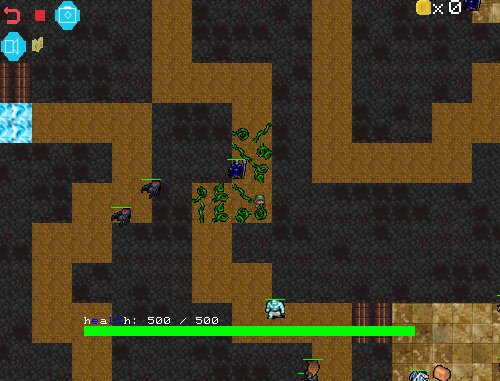
\includegraphics{img/preview.png}
		\cnenfigcaption{游戏截图}{game screenshot}
		\label{preview}
	\end{figure}
\begin{enumerate}
	\item UI框架:游戏最初基于jw04的框架,想利用AsciiFont提供的图形组合设计复杂的游戏角色,做一个类似飞机大战的FPS游戏。为此在jw04的基础上设计了一个可以移动玩家观察视角和引入大地图的scene-view结构。jw05发布后,将已经做的部分改成UI框架,截止目前,UI框架可以完成鼠标、键盘事件在组件之间传递、提供监听键盘事件的接口、响应窗口调整大小、自动布局、背景等功能。
	\item 随机地图:为避免单一关卡带来的疲倦感和避免关卡设计耗费大量时间,我决定做一个随机地图的生成程序。在参考网上相关思路后,借助jw04的迷宫生成模块实现了一个随机地牢生成程序。
	\item 网络通信:多人游戏时,游戏状态以房主为准。同步操作采用帧同步和状态同步,游戏动作同步主要由帧同步。状态同步会定期由服务端或者发生网络波动的客户端发起。游戏不需求同时开始,在房主处于多人游戏状态下,其它玩家可以随时加入游戏。
	\item 游戏设计:
	\begin{itemize}
		\item 游戏角色本身不是一个线程,但是每一个角色都由一个controller控制。
		\item 在脱离战斗和锁定敌人的情况下,怪物行为具有随机性, 怪物技能CD
		\item 多种怪物分工明确
		\item 对控制角色的控制器写成线程,解决键盘操作卡手的问题。
		\item 实现了所有生物通用的增益系统,玩家自机角色可以捡拾使用宝箱掉落的Buff,并在短时间内获得某一方面的属性强化
		\item 实现地图出口,可交互宝箱等可交互对象
	\end{itemize}
	\item 存档功能:所有需要存档的对象实现统一接口,实现从Object到JSON字符串的互相转换。将地图和游戏信息、creature信息等打包为json字符串作为游戏存档,并提供管理存档的UI界面。
	\item 截图和录制:利用该项目已有的UI框架,自定义组件获取每一帧图像并转换格式输出。
\end{enumerate}
\section{设计理念}
\subsection{物体}
图\ref{graphics.pu}是有关游戏图形组件的结构图\par
为了提高代码复用率,大部分逻辑代码实现在Creature,Thing,Effect,Bullet等几个父类里,它们的衍生子类大多只有资源和参数定制。其中,项目还设计了包括controllable,PFrameKeyLisnter,GameThread等接口用来表示不同的功能模块,某个类实现了某个模块即代表支持且需要进行对应功能的操作,这有利于系统其它部分从一堆Thing类型的变量识别需要的变量。例如,World会在存档是将所有为StatedSavable(状态可以被保存为json格式)实例的Thing类型变量保存至存档中。因为Creatrue实现了StatedSavable接口,意味着后来的所有Creature子类自创建就默认拥有写进存档的功能,不需要额外代码。
	\begin{figure}[!t]
		\centering
		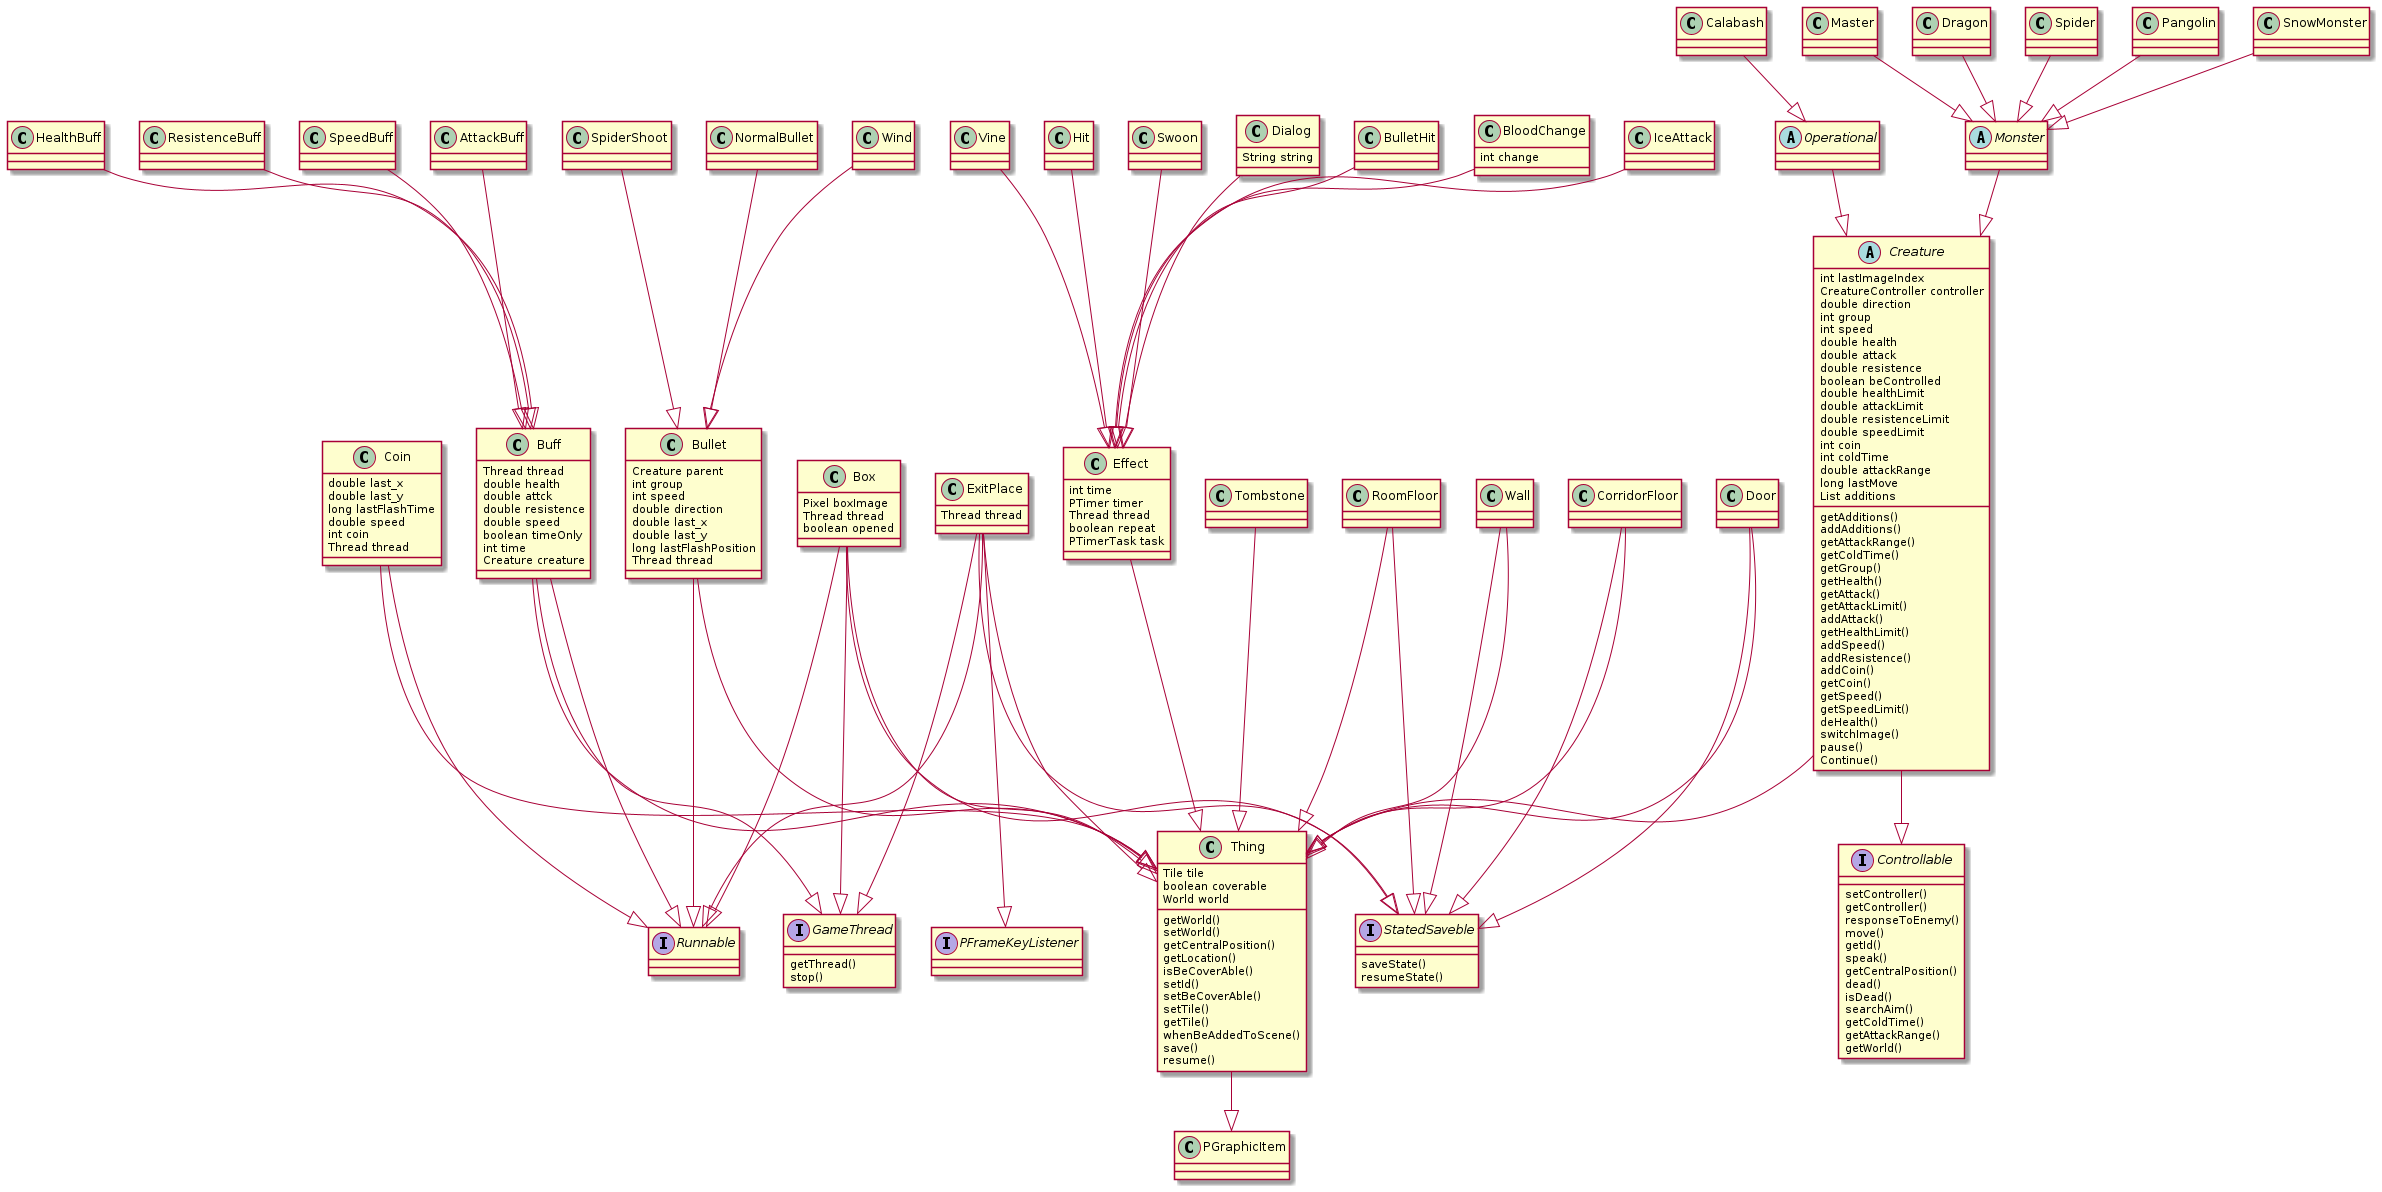
\includegraphics[width=1.0\textwidth]{img/graphics.png}
		\cnenfigcaption{类图}{class picture}
		\label{graphics.pu}
	\end{figure}
\subsection{UI}
因为jw04原来的框架局限太大,无法满足自定义多种形状和大小的图形需求,所以最终做成了UI框架。可惜由于底层渲染的方式是由一个一个像素计算和操作,后期也难以用上其它方式改进,加上需要不断刷新,UI框架反而成为了性能的最大拖累。UI部分模块可以用来快速创建一些布局限制条件简单的可缩放UI界面。因为所有UI组件都是PWidget子类,因此,各种控件之间组合自由度很高;在继承PWidget(最原始的UI组件)并通过重写部分方法,也可以自行编写定制的组件。
\subsection{NetWork}
联机模式结构图\ref{jw-network.drawio}\par
	\begin{figure}
		\centering
		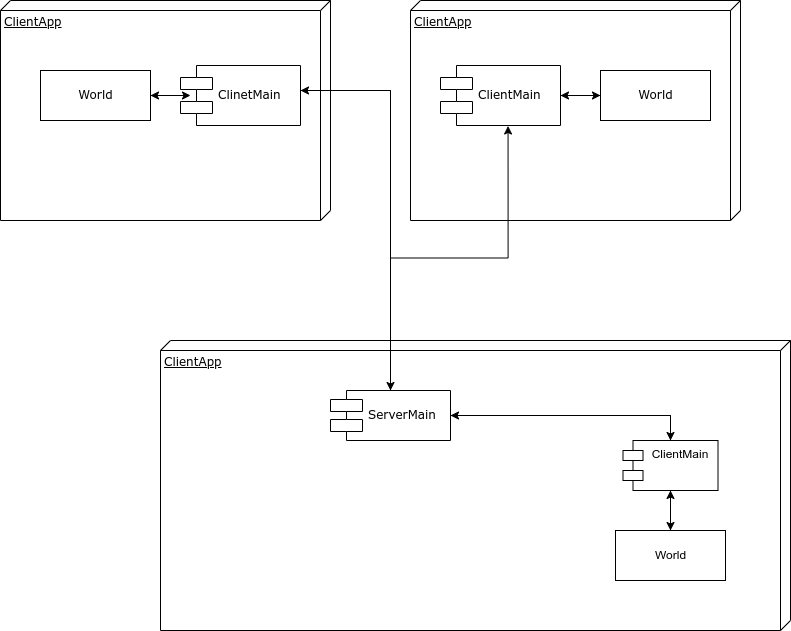
\includegraphics[width=1.0\textwidth]{img/jw-network.drawio.png}
		\cnenfigcaption{联机模式结构图}{multi mode model}
		\label{jw-network.drawio}
	\end{figure}
联机模式的同步策略同时采用帧同步和状态同步的方式。帧同步:系统每20ms收集一次来自所有客户端的输入信息,并打包广播给所有客户端,进行这一帧的运算;状态同步:当某个客户端发生丢帧事件后,会向服务端发送状态同步请求,同时服务端每1秒也会自动产生一次请求,状态同步时,服务端先向主客户端发送请求获取主客户端的状态信息,再向其它客户端进行广播。\par
网络部分被设计为多人模式下,启动一个多人游戏时,系统会创建一个客户端和一个服务端(默认监听9000号端口)并进行连接。服务端会将这个首先连接的客户端作为主客户端,并生成游戏存档并发送给主客户端。游戏中的一切实际状态以主客户端为主,其它客户端的任何不同步会在状态同步中缩小或消除。\par 
客户端可以通过输入ip地址连接服务端。收到请求后,如果连接人数没有超过限制,服务端会生成一个新的角色连同游戏存档发送给客户端进行游戏初始化,同时通知主客户端有新的玩家加入世界。在经过一次状态同步后,新加入的客户端会与其它客户端同步,并进入正常运行。\par
网络故障和客户端关闭处理。客户端和服务端在遇到网络障碍或者关闭时会自动退出游戏或者发送玩家退出游戏的命令。
\subsection{存档}
游戏提供了专门用于对象状态和json对象之间转换的接口:\\
\begin{lstlisting}
public interface StatedSavable {
	public JSONObject saveState();
	public void resumeState(JSONObject jsonObject);
}
\end{lstlisting}
\par
一个典型的Creature对象生成的json字符串:\\
\begin{lstlisting}
{
	"beCoverAble": false,
	"attack": 20.0,
	"health": 400.0,
	"position": "{1980,620}",
	"id": 10493,
	"class": "game.graphic.creature.monster.SnowMonster",
	"resistance": 0.1,
	"speed": 2,
	"group": 1,
	"coin": 1
}
\end{lstlisting}
\par
在游戏保存时,程序对于在world里的StatedSaveable实例获取JSONObject;在游戏记载时,获取json字符串中的class名称创建Object并读取jsonObject恢复状态。将对象的保存和恢复交给具体的对象解决,而大多数的保存工作这些对象的基类就已经完成,这样避免了在加载和保存模块里大量复杂的逻辑代码,同时这些对象State恢复和保存的特性也可以为网络中的状态同步提供便利。
\section{技术问题}
\subsection{并发控制}
为了综合考虑程序正确性和并发效率的问题。UI部分的刷新操作是不会对对象进行上锁操作;对于World中对象的移动等操作都是由不同的线程中完成,可能因为多线程同步问题产生冲突,会首先试探目标资源的可用性。如果可用,则先上锁,再试探一次,如果可行就进行下一步操作。
\subsection{资源节省}
因为游戏生成大地图的需求,需要同时生成的对象数量非常之多,不得以采取多种方法节省内存开销:
\begin{itemize}
	\item 对于已经加载过的图片资源进行缓存,以减少磁盘IO次数,加快运行速度
	\item 对于大部分Thing的子类,如果可以共用图片资源,都不会再生成一份图形资源,而是所有类共用资源
	\item 在单机模式下,地图上的怪物不会被一次性加载出来,特制的维护型thread会保证只有角色周围一定范围内的怪物被加载。
	\item 为了提高world的渲染速度,地图被切成一块块方格。单次渲染中,只有在当前视野内的方格内的对象会被渲染。
\end{itemize}
\subsection{通信效率}
为了提高通信效率,我在主流的帧同步和状态同步中选择了实时性更强、视觉效果更好但更难实现的帧同步。因为如果采用状态同步,同时需要同步的还有大量的子弹和创造物,对网络压力更大;而采用帧同步可以只同步角色和怪物的动作请求,可以减少通信量。同时更重要的是:状态同步下游戏人物的帧数本质取决于一秒内同步的次数,而帧同步传递操作,在本地演算动作,在程序性能好的情况下,帧同步的帧数和观感要远强于状态同步。但纯粹的帧同步往往会因为网络延迟等原因导致不同客户端之间的数据产生差异,最终在某些边缘情况下导致差异被急剧放大。所以,在通信方面,程序采用了帧同步和状态同步的方式。\par 
在通信方面,为了防止因为服务端因为挨个发包阻塞和网络波动导致不同客户端收到包的时间差异过大或者由于单个客户端网络波动导致全部客户端卡顿。单次的发送请求被作为单个线程提交给线程池执行,确保不会阻塞;\par 
\section{工程问题}
\subsection{运用的设计模式}
\begin{itemize}
	\item 单例模式:多人模式下的Client端采用单例模式,保证单个程序只有一个Client端
	\item 工厂方法:程序中Position,Pixel,Message都采用了静态工厂方法,它的好处在于,方法内部可能会使用new创建一个新的实例,但也可能直接返回一个缓存的实例。对于调用方来说,没必要知道实例创建的细节。
	\item 享元模式:大部分的Thing子类内部通过静态变量共享同一份图形资源,避免不必要的资源加载。
	\item 命令模式:Client和Server调用发送Message只是委托其它线程进行发送行为;
	\item 观察者、状态模式:大部分UI组件在size变化后会调用特定的函数处理变化,重新渲染缓存的图像等工作。同时,将size变化传递给它的孩子组件,引起其它组件的变化。
	\item 备忘录模式:可保存状态的对象在游戏存档和加载时与json对象之间的互相转换。
\end{itemize}
\subsection{工程方法}
\begin{itemize}
	\item 采用单元测试,确保单个子功能功能正常
	\item 程序模块划分清晰,在完成不同的模块合并后进行大量集成测试模块是否正常工作;
	\item 采用回归测试,确保程序在不断迭代的 情况下功能的正常;
\end{itemize}
\end{document}